\documentclass[../hydrozoa.tex]{subfiles}
\graphicspath{{\subfix{../images/}}}
\begin{document}

\chapter{L1 multisig regime}%
\label{h:l1-multisig-regime}%

Every Hydrozoa head uniquely corresponds to its peers' public key hashes.
In the L1~multisig~regime, the head's native script simply requires signatures from all these public key hashes:%
\footnote{We use similar notation to the Cardano ledger library \citep{IntersectMBOCardanoLedgerV117402025}, simplifying for readability.
In that library, native scripts are sometimes called ``timelock'' scripts.}
\begin{equation*}
\begin{split}
  \T{headNativeScript} &:: \T{Set} \; \T{PubKeyHash} -> \T{Timelock} \\
  \T{headNativeScript} &\coloneq
    \T{AllOf} \;.\; \T{map} \; \T{Signature}
\end{split}
\end{equation*}

We could end this chapter here, as no other conditions are enforced by L1 scripts in the multisig regime.
However, we will describe this regime's expected states and transitions, which the Hydrozoa L2 consensus protocol enforces while the peers engage with it (\cref{h:l2-consensus-protocol}).%
\footnote{Of course, the peers can always manually override the L2 consensus protocol by unanimous consent.}

\section{Utxo state}%
\label{h:l1-multisig-utxo-state}%

In the multisig regime, a head's entire L1 state resides in utxos at its native script address.
\begin{equation*}
  \T{MultisigHeadState^{L1}} \coloneq \left\{
  \begin{array}{lll}
    \T{treasuryUtxo} &::& (\T{OutputRef}, \T{Output^{L1}}) \\
    \T{depositUtxos} &::& \T{UtxoSet^{L1}} \\
    \T{rolloutUtxos} &::& \T{UtxoSet^{L1}}
  \end{array}\right\}
\end{equation*}

\begin{figure}[H]
\begin{center}
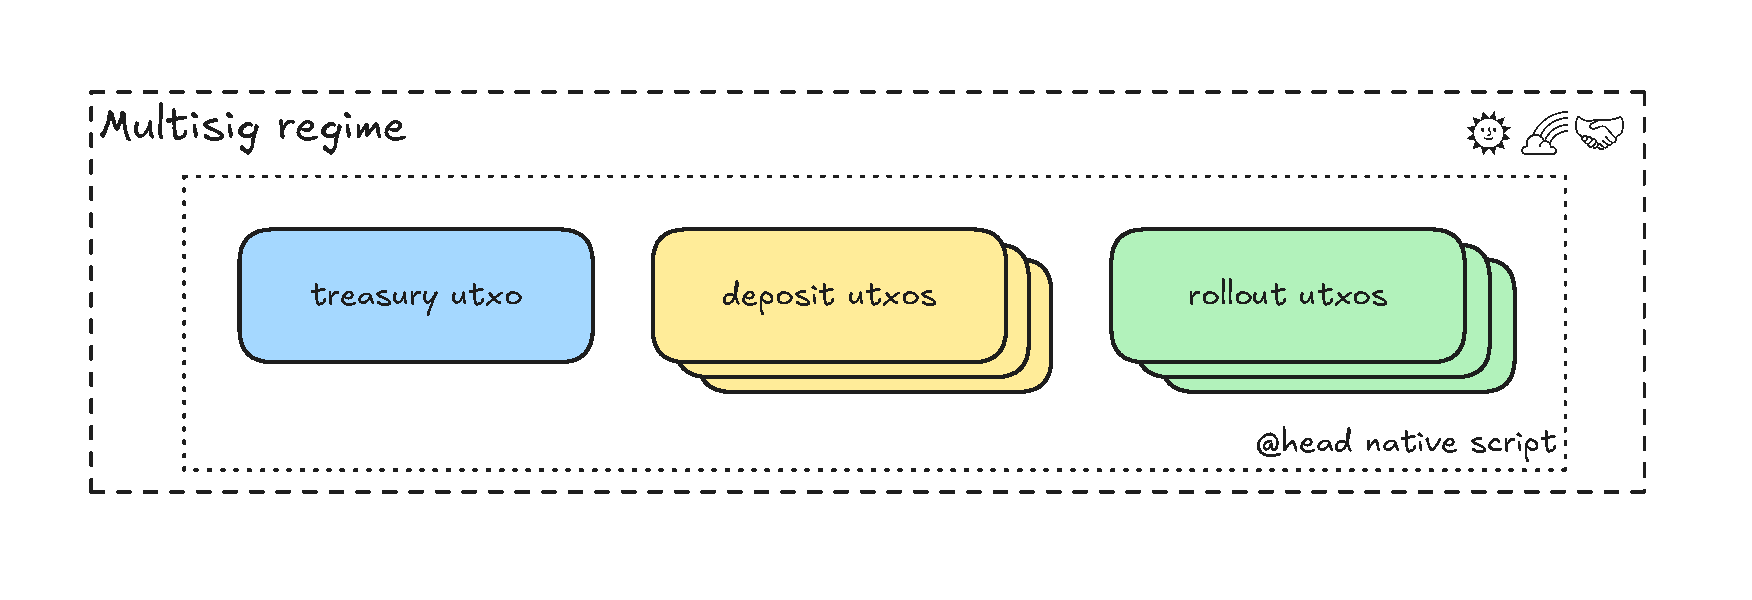
\includegraphics[width=\txDiagramScale\linewidth]{\subfix{../images/tx-diagram/1-multisig-regime-utxo-state.pdf}}
\end{center}
\caption[Multisig regime utxo state on L1.]{The L1 utxo state of the multisig regime.}
\label{fig:utxo-state-multisig-regime}
\end{figure}

Among these utxos, the head's treasury utxo is uniquely identified as the one holding the head's beacon token:
\begin{enumerate}
  \item The policy ID corresponds to the head's native script (in minting policy form).
  \item The first four bytes of the asset name are equal to the CIP-67
    \citep{AlessandroKonradThomasVellekoopCIP67AssetName2022}
    prefix for class label \headBeaconToken{}, which corresponds to Hydrozoa head beacon tokens.%
    \footnote{We chose \headBeaconToken{} because it spells ``HYDR'' (short for Hydra/Hydrozoa) on a phone dial pad.}
  \item The last 28 bytes of the asset name are equal to the Blake2b-224 hash (\codeMath{\mathcal{H}_{28}}) of the utxo nonce spent in the head's initialization transaction (\cref{h:l1-multisig-initialization}).
\end{enumerate}
No other utxo at the head's native script address should hold any tokens that meet the policy ID and CIP-67 prefix conditions above.
In other words, there must only be one head at the address.%
\footnote{It may seem redundant to use a 28-byte unique nonce in the beacon token's asset name, given that only one head is allowed per native script address at any given time.
  However, the unique nonce helps distinguish between different heads that may exist at the same address across time.}

The treasury utxo must have this datum:
\begin{equation*}
  \T{MultisigTreasuryDatum} \coloneq \left\{
    \begin{array}{lll}
      \T{utxosActive}  &::& \mathcal{RH}_{32} \; \T{UtxoSet^{L2}} \\
      \T{versionMajor} &::& \T{UInt} \\
      \T{params} &::& \mathcal{H}_{32} \; \T{ParamsConsensusL2}
    \end{array}\right\}
\end{equation*}
These fields are interpreted as follows:
\begin{description}
  \item[active utxos.] A 32-byte Merkle root hash (\codeMath{\mathcal{RH}_{32}}) of the L2 ledger's active utxo set, as of the latest major L2 block settled on L1 (\cref{h:l1-multisig-settlement}).
  \item[major version.] The version number of the latest major L2 block settled on L1.
  \item[params.] A 32-byte Blake2b-256 hash (\codeMath{\mathcal{H}_{32}}) of the head's L2 consensus parameters (\cref{h:l2-head-state}).
\end{description}

Non-treasury utxos at the head's native script address are recognized as follows:
\begin{itemize}
  \item A rollout utxo holds a rollout beacon token of the head's minting policy, with CIP-67 prefix \headRolloutToken{}.%
    \footnote{We chose \headRolloutToken{} because it spells ``ROLL'' (short for rollout) on a phone dial pad.}
    It is a no-datum output of a settlement, finalization, or rollout transaction.
    It is transient---quickly spent in a subsequent rollout transaction.
  \item A deposit utxo has a datum with the \code{DepositDatum} type (\cref{h:l1-multisig-deposit}).
\end{itemize}
  
\section{Initialization}%
\label{h:l1-multisig-initialization}%

Before initializing a Hydrozoa head, the peers should agree on the L2 consensus parameters they want to use (\cref{h:l2-consensus-protocol}).
Initialization is achieved with a single transaction, multi-signed by all the peers, that:
\begin{itemize}
  \item Mints the head's beacon token.
  \item Spends the utxo nonce reference by hash in the last 28 bytes of the beacon token's asset name.
  \item Creates the treasury utxo at the head's native script address, placing the beacon token into it (with min-ADA) with this datum:
    \begin{equation*}
    \begin{split}
      \T{initMultisigTreasuryDatum} &:: \mathcal{H}_{32} \; \T{ParamsHead} -> \T{MultisigTreasuryDatum} \\
      \T{initMultisigTreasuryDatum} &\; \T{initParams} \coloneq \left\{
        \begin{array}{lll}
          \T{utxosActive} &=& \mathcal{RH}_{32} \; \varnothing \\
          \T{versionMajor} &=& 0 \\
          \T{params} &=& \T{initParams}
        \end{array}\right\}
    \end{split}
    \end{equation*}
\end{itemize}

\begin{figure}[H]
\begin{center}
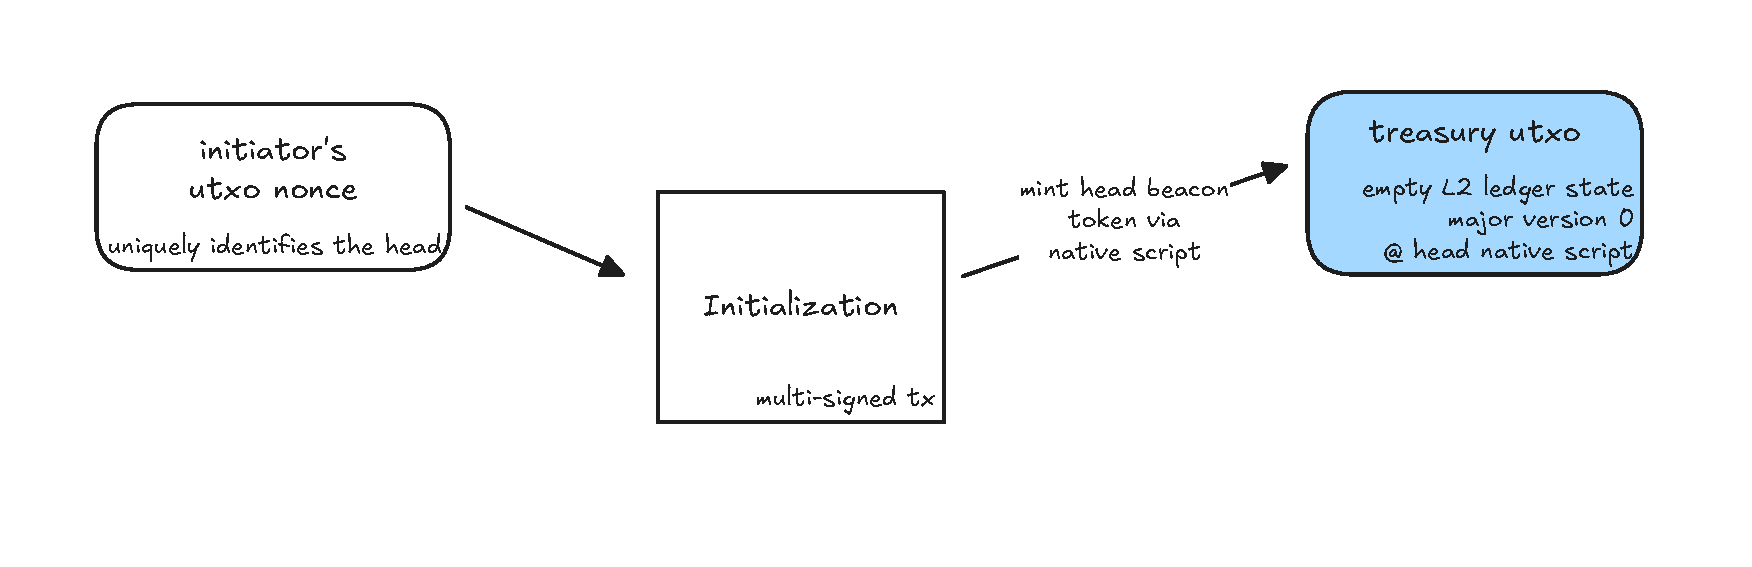
\includegraphics[width=\txDiagramScale\linewidth]{\subfix{../images/tx-diagram/2-initialization-tx.pdf}}
\end{center}
\caption[Multisig regime: Initialization tx.]{The Hydrozoa head's peers initialize its treasury utxo with an empty L2 ledger.}
\label{fig:tx-initialization}
\end{figure}

\section{Deposit}%
\label{h:l1-multisig-deposit}%

Peers can deposit funds into a Hydrozoa head by sending utxos to its native script address, specifying their instructions in this datum type:
\begin{equation*}
  \T{DepositDatum} \coloneq \left\{
  \begin{array}{lll}
    \T{address} &::& \T{Address^{L2}} \\
    \T{datum} &::& \T{Maybe \; Datum^{L2}} \\
    \T{deadline} &::& \T{PosixTime} \\
    \T{refundAddress} &::& \T{Address^{L1}} \\
    \T{refundDatum} &::& \T{Maybe \; Datum^{L1}}
  \end{array}\right\}
\end{equation*}

In this datum, the depositor instructs the peers to absorb the deposit into the treasury via a settlement transaction (\cref{h:l1-multisig-settlement}) before the \code{deadline}, or else to refund it to the depositor (\cref{h:l1-multisig-refund}) if it will not be absorbed before the \code{deadline}.

The \code{address} and \code{datum} fields define the address and datum at which the utxo in the L2 ledger should be created if the deposit is absorbed into the head's treasury.
The new utxo in the L2 ledger should contain the same funds as the deposit utxo.

The \code{refundAddress} and \code{refundDatum} fields define the address and datum to which the deposit's funds should be sent on L1 if the deposit is refunded.
The funds in the deposit must be sufficient to pay for the refund transaction cost and create the refund utxo.

\begin{figure}[H]
\begin{center}
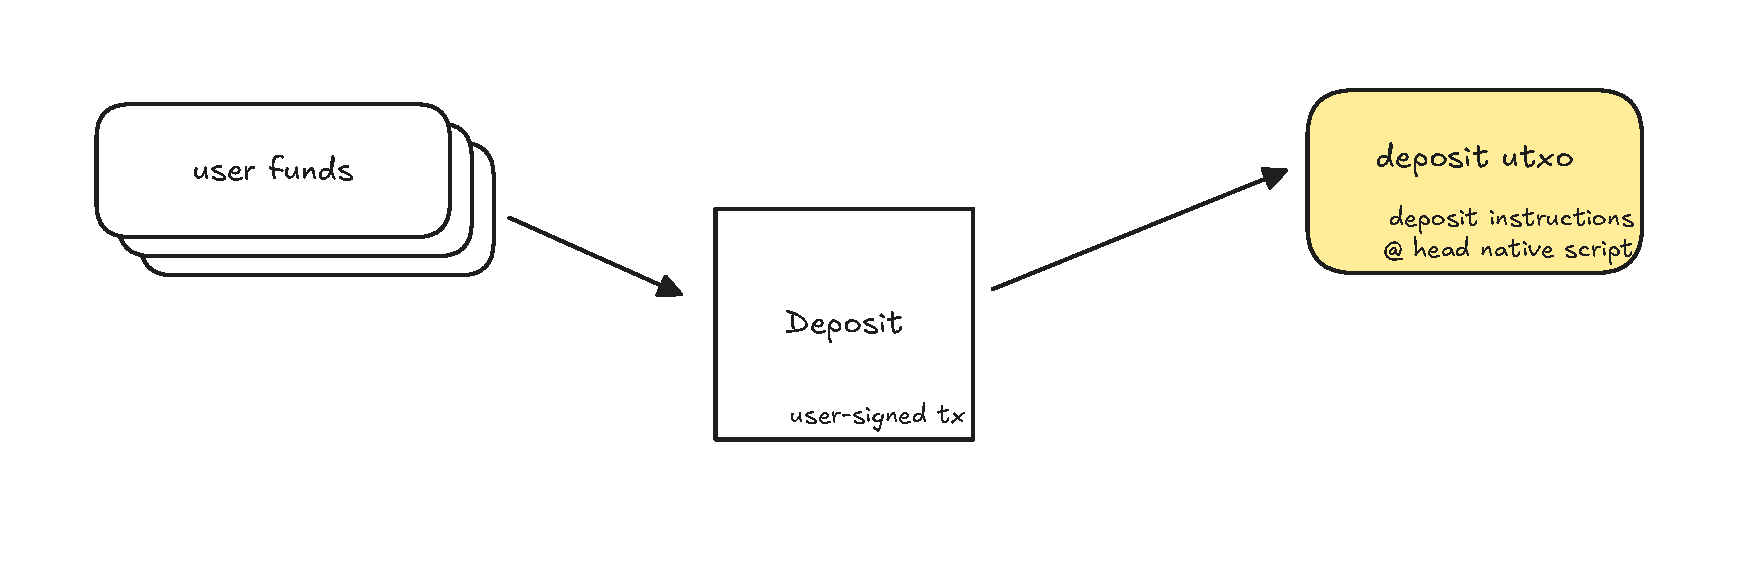
\includegraphics[width=\txDiagramScale\linewidth]{\subfix{../images/tx-diagram/3-deposit-tx.pdf}}
\end{center}
\caption[Multisig regime: Deposit tx.]{A user places some funds and instructions into a deposit utxo for a Hydrozoa Head.}
\label{fig:tx-deposit}
\end{figure}

\section{Refund}%
\label{h:l1-multisig-refund}%

A refund is a transaction, multi-signed by all peers, that sends a deposit utxo's funds to the deposit's \code{refundAddress} and \code{refundDatum}.
While the peers follow the L2 consensus protocol, they will automatically multi-sign and submit refund transactions for all deposits not absorbed before their deadline.%
\footnote{To minimize uncertainty from L1 rollbacks, the L2 consensus protocol will not attempt to absorb a deposit unless sufficient time remains before its deadline.
This safety margin is controlled by an offchain consensus parameter (\cref{h:l2-consensus-parameters}).}

However, a depositor should obtain the other peers' signatures for a post-dated refund transaction before submitting the deposit transaction to Cardano.
This transaction's validity interval should start at the deposit's \code{deadline}.
Doing so ensures that the depositor can still retrieve the deposited funds if they have not been absorbed by the deadline, even if the other peers stop responding.

The L2 consensus protocol (\cref{h:l2-consensus-on-refunds}) allows peers to obtain multi-signed post-dated refund transactions before posting their deposits on L1.
It also allows them to immediately refund any deposits that its rules disqualify from being absorbed into the treasury.

\begin{figure}[H]
\begin{center}
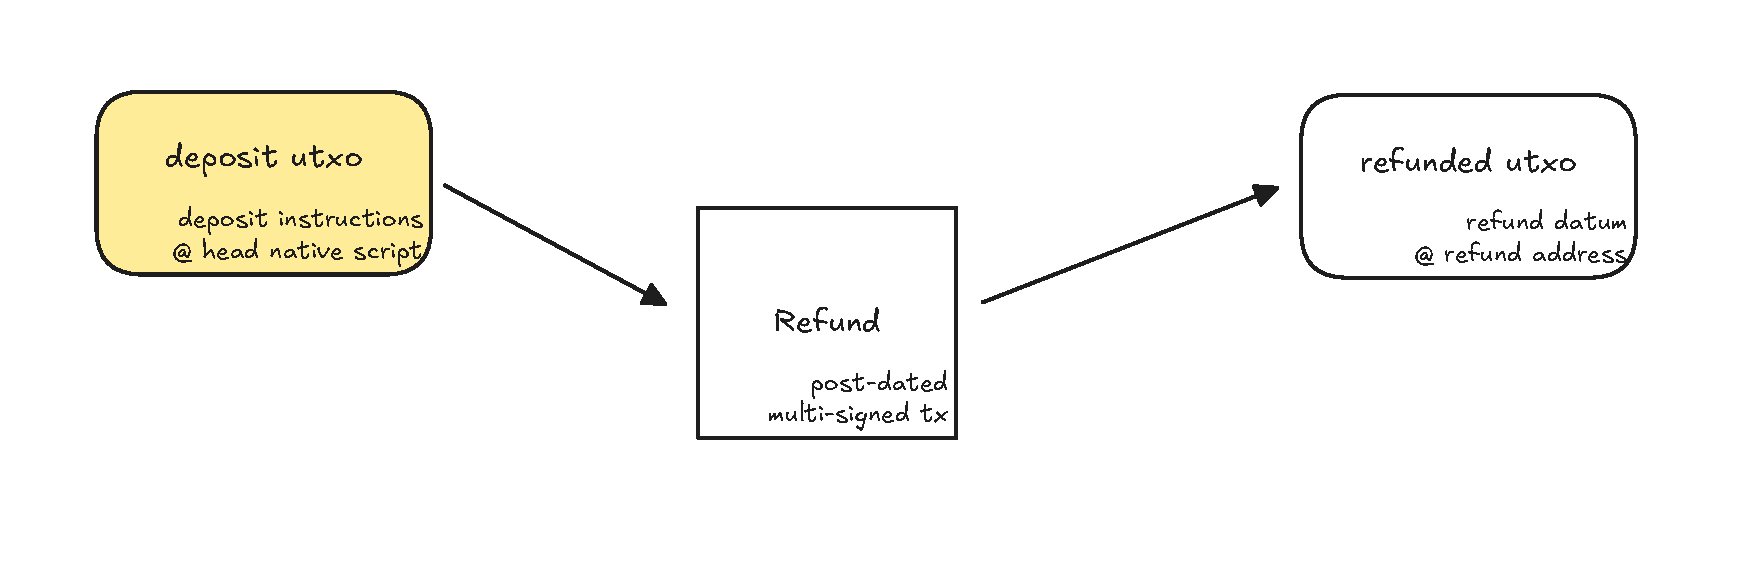
\includegraphics[width=\txDiagramScale\linewidth]{\subfix{../images/tx-diagram/4-refund-tx.pdf}}
\end{center}
\caption[Multisig regime: Refund tx.]{The peers refund the deposit if it isn't absorbed into the treasury before the user's deadline.}
\label{fig:tx-refund}
\end{figure}

\section{Settlement}%
\label{h:l1-multisig-settlement}%

A settlement is a transaction, multi-signed by all peers, that absorbs deposits into a Hydrozoa head's treasury and pays out withdrawals out of the treasury based on a major L2 block (\cref{h:l2-blocks}).%
\footnote{A block is ``major'' if it confirms new deposits or withdrawals that were not confirmed in the preceding blocks.}
It also updates the \code{versionMajor} and \code{utxosActive} fields of the \code{MultisigTreasuryDatum} to the corresponding fields in the major L2 block while keeping the \code{params} field unchanged.

The absorbed deposit utxos are spent inputs in the settlement transaction.
This means that Cardano's transaction size limit constrains the number of deposits settled per major L2 block.

On the other hand, the number of withdrawals per major L2 block is unconstrained.
The withdrawn utxos of the major L2 block are paid out via outputs of the settlement and rollup transactions, in the ascending order of their output references in the L2 ledger.

The assignment of L2 withdrawn utxos to L1 outputs of the settlement and rollout transactions is handled by Hydrozoa's deterministic rollout algorithm (\cref{h:deterministic-rollout-algorithm}).
The settlement transaction greedily pays out as many withdrawals as it can, using the transaction size remaining after fitting the deposit inputs and the fixed transaction overhead.
It outputs the remaining withdrawals' aggregate funds as a single rollout utxo, sent to the head's native script address without a datum.
Rollout transactions iteratively pay out more utxos from the rollout utxo, until all withdrawals are settled (\cref{h:l1-multisig-rollout}).

\begin{figure}[H]
\begin{center}
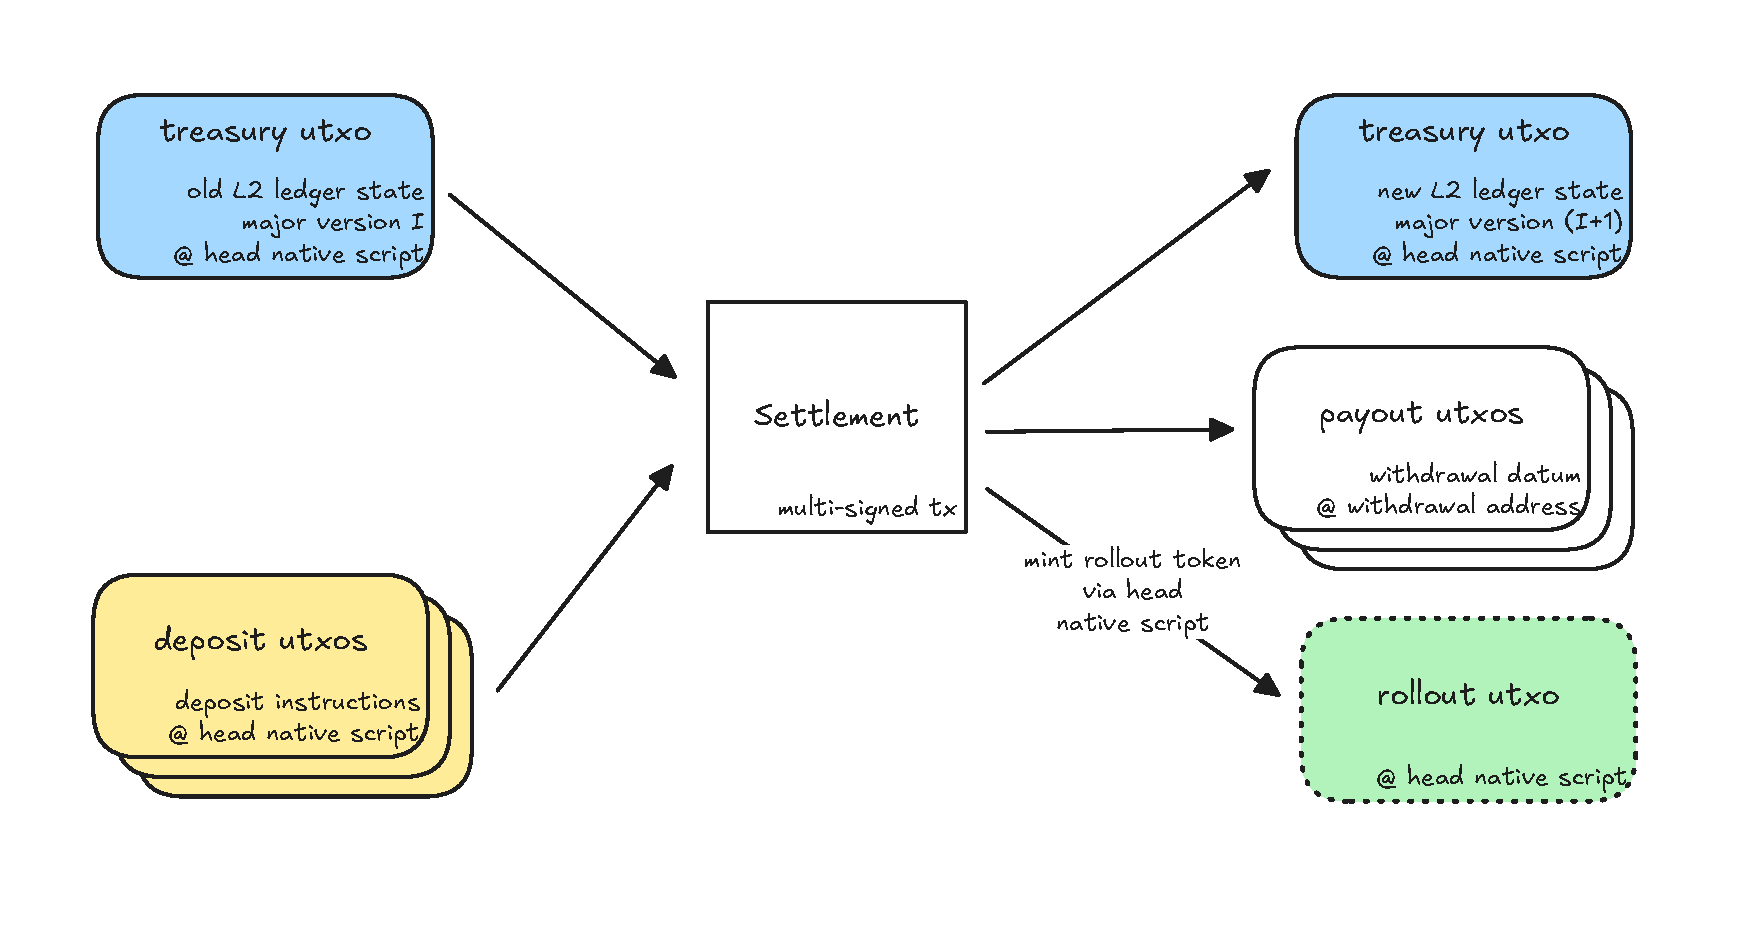
\includegraphics[width=\txDiagramScale\linewidth]{\subfix{../images/tx-diagram/5-settlement-tx.pdf}}
\end{center}
\caption[Multisig regime: Settlement tx.]{The peers absorb some deposits and pay out some withdrawals from the head's treasury.
A rollout utxo can be produced to defer payout of some withdrawals for later.}
\label{fig:tx-settlement}
\end{figure}

\section{Finalization}%
\label{h:l1-multisig-finalization}%

The finalization transaction is similar to the settlement transaction, except that:
\begin{itemize}
  \item It burns the head's beacon token.
  \item It spends the head's treasury utxo without outputting a new treasury utxo.
  \item It does not absorb any deposits.
  \item It withdraws all utxos in the final L2 block's ledger, including those in the active utxo set, using rollout transactions if necessary.
\end{itemize}

After the finalization transaction deals with the treasury and immediate/post-dated refund transactions deal with the unabsorbed deposits, no trace of the Hydrozoa head should be left in the L1 ledger.
Any other utxos that remain at the head's native script address---assumed to be unrelated to the head---can be manually spent by the peers.

\begin{figure}[H]
\begin{center}
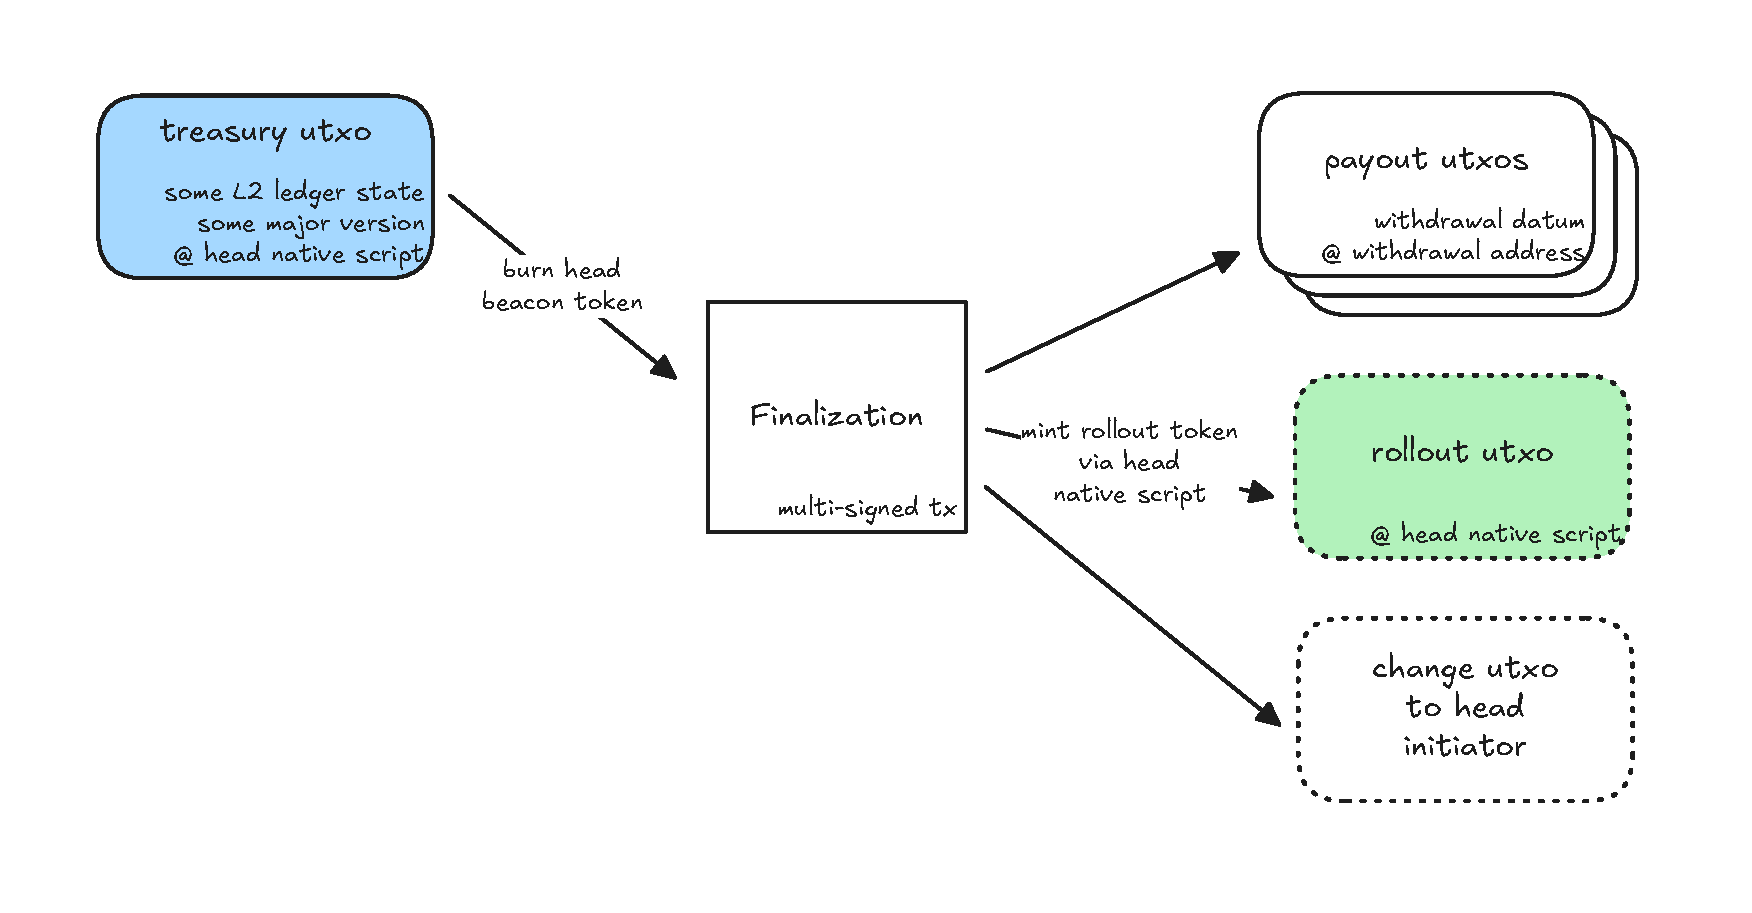
\includegraphics[width=\txDiagramScale\linewidth]{\subfix{../images/tx-diagram/6-finalization-tx.pdf}}
\end{center}
\caption[Multisig regime: Finalization tx.]{The peers pay out all remaining funds from the head's treasury.
A rollout utxo can be produced to defer the payout of some withdrawals for later.}
\label{fig:tx-finalization}
\end{figure}

\section{Rollout}%
\label{h:l1-multisig-rollout}%

The rollout utxo is spent in a rollout transaction, paying out some more withdrawals, and outputting a new rollout utxo with the aggregate funds of the rest of the withdrawals, if any remain.
Further rollout transactions spend the shrinking rollout utxo, until all the withdrawals have been paid out (\cref{h:deterministic-rollout-rollouts}).

\begin{figure}[H]
\begin{center}
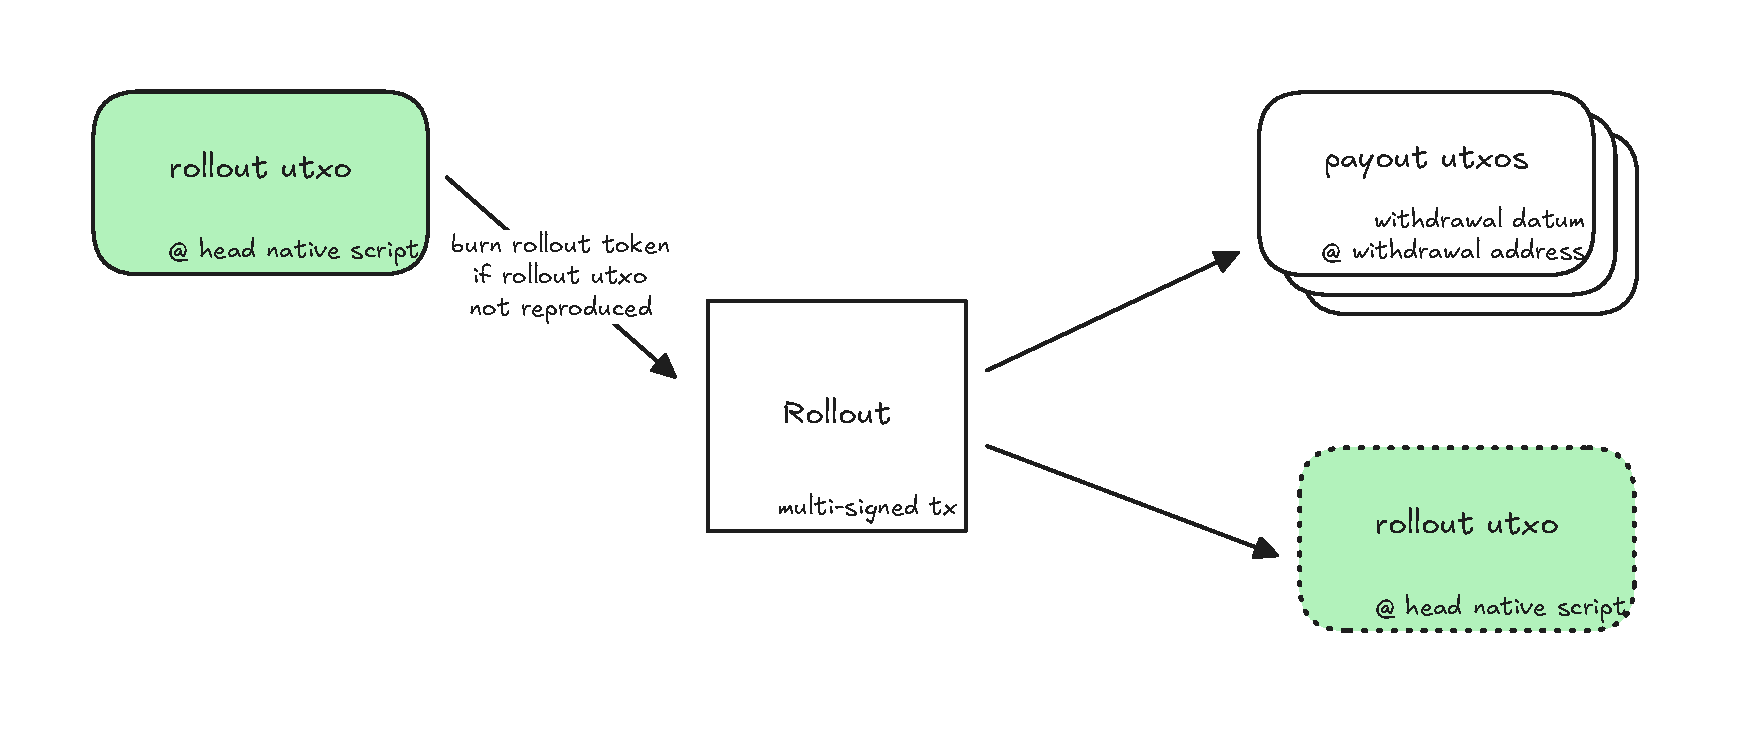
\includegraphics[width=\txDiagramScale\linewidth]{\subfix{../images/tx-diagram/7-rollout-tx.pdf}}
\end{center}
\caption[Multisig regime: Rollout tx.]{The peers pay out some withdrawals out of a rollout utxo, possibly leaving some for later payout.}
\label{fig:tx-rollout}
\end{figure}

\end{document}
